\section*{Triángulo de Pascal}

En las matemáticas, el triángulo de Pascal es una representación de los
coeficientes binomiales ordenados en forma de triángulo. Es llamado así en honor
al filósofo y matemático francés Blaise Pascal, quien introdujo esta notación en
1654, en su Tratado del triángulo aritmético.

\newcommand{\pasc}[2]{
	\pgfkeys{/pgf/fpu}
	\pgfmathparse{round(#1!/((#1-#2)!*#2!))}
	\pgfmathfloattoint{\pgfmathresult}
	\pgfmathresult
}

\begin{figure}[h]
	\centering
	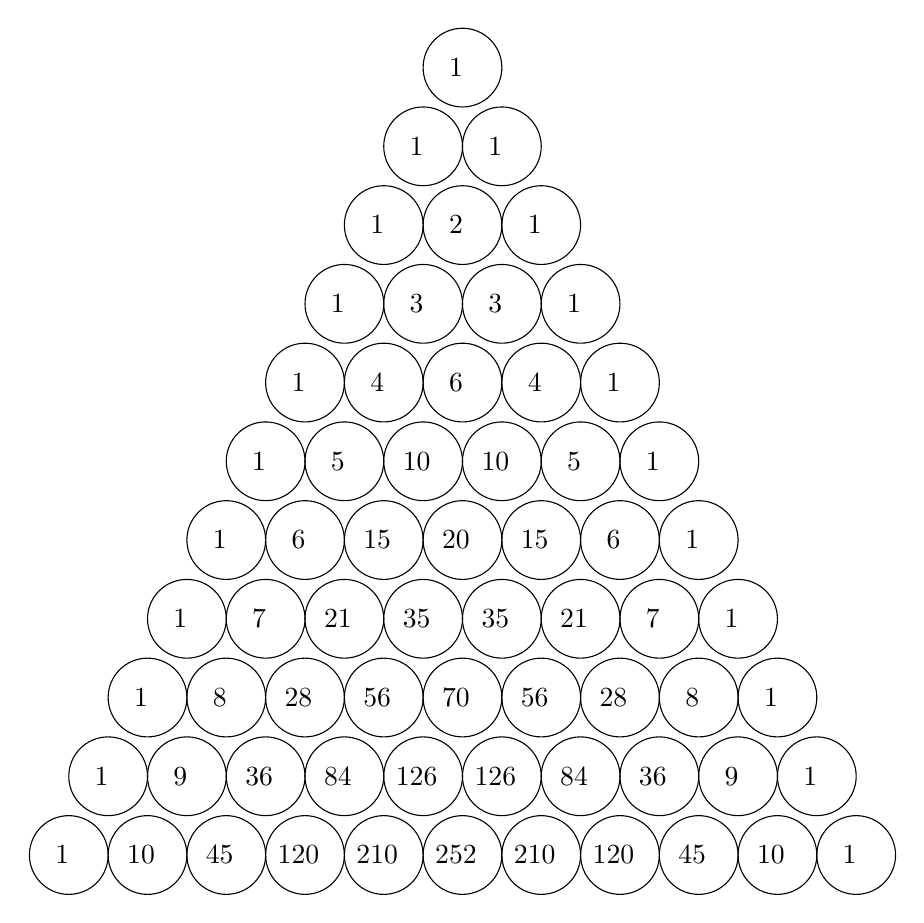
\begin{tikzpicture}
	\pgfmathsetmacro{\N}{10};
	\foreach \i in {0,...,\N}{
		\foreach \j in {0,...,\i}{
			%\pgfmathtruncatemacro{\var}{\pasc{\i}{\j}}
			\node at ({-0.5*\i+\j-0.2},-\i){\pasc{\i}{\j}};
			
			%\ifthenelse{\pasc{\i}{\j}=}{then clause}{else clause}
			% \draw ({-0.5*\i+\j-0.5},-\i+0.5) rectangle
			% ({-0.5*\i+\j-0.5},-\i-0.5);
			\draw ({-0.5*\i+\j},-\i) circle (0.5) ;
		}
	}
	\end{tikzpicture}
	\caption{Triángulo de Pascal para n=10}
	\label{fig:pascalTriangle}
\end{figure}

Este triángulo fue ideado para desarrollar las potencias de binomios.

La fórmula del binomio de Newton desarrolla los coeficientes de cada fila en el
triángulo de Pascal. Es por esto que existe una estrecha relación entre el
triángulo de Pascal y el binomios de Newton.

\subsection*{Propiedades del triángulo de Pascal}

Algunas de las propiedades más representativas del triángulo de Pascal son las
siguientes:

\begin{itemize}
	\item Cada número es la suma de los dos números encima de él.
	\item Todos los números exteriores son iguales a 1.
	\item El triángulo de Pascal es simétrico.
	\item La primera diagonal muestra los números de conteo.
	\item Las sumas de las filas dan las potencias del 2.
	\item Cada fila da los dígitos de las potencias del 11.
	\item Cada elemento representa a la combinación , en donde, m es la fila del elemento y n es la posición del elemento en la fila.
	\item Cada fila representa a los coeficientes binomiales.
	\item Los números Fibonacci están a lo largo de las diagonales.
\end{itemize}

\subsection*{Patrones del triángulo de Pascal}

\subsubsection*{Suma de las filas}

Una de las propiedades interesantes del triángulo es que la suma de los números
en una fila es igual a $2^n$, en donde, n corresponde al número de la fila. Por
ejemplo, tenemos:

$ 1 = 1 = 2^0 $ \\
$ 1 + 1 = 1 = 2 = 2^1 $ \\
$ 1 + 2 = 1 = 4 = 2^2 $\\

como se puede observar en la Fig. (\ref{fig:pascalTriangle})

\subsubsection*{Números primos en el triángulo}

Otro patrón visible en el triángulo se relaciona a los números primos. Si es que
una fila empieza con un número primo o es una fila con número primo, todos los
números que están en esa fila, sin incluir al 1, son divisibles para ese número
primo.

Si es que miramos a la fila 5 (1, 5, 10, 10, 5, 1) podemos ver que el 5 y el 10
son divisibles por 5. Sin embargo, para una fila compuesta como la fila 8 (1, 8,
28, 56, 70, 56, 28, 8, 1), 28 y 70 no son divisibles por 8.

\subsubsection*{Sucesión de Fibonacci en el triángulo}
En el triángulo de Pascal se puede apreciar una relación entre un modo de sumar
las diagonales y la sucesión de Fibonacci. Los primeros términos de esta
sucesión son: $1,1,2,3,5,8,13,21,34,55$ como se puede apreciar en la Fig.
(\ref{fig:pascalTriangle}).

\subsubsection*{Expansión binomial con el triángulo de Pascal}

El triángulo de Pascal define a los coeficientes que aparecen en las expresiones
binomiales. Eso significa que la fila n del triángulo de Pascal contiene a los
coeficientes de la expresión expandida del binomio $(x+y)^n$.